\documentclass{article}
\usepackage{amsmath}
\usepackage{amssymb}
\usepackage{graphicx} 

\title{VAN final project report}
\date{2020-05-01}
\author{Shai Guendelman, Avnum Hanuhov}

\begin{document}
	% this is how to comment with '%'
	% this produces the title in a single front page
	\maketitle
	\newpage
	
	% sections, subsections, and subsubsections are of 
	% different topics.
	% paragraphes and subparagraphes are not numbered
	% this is a section with latex examples. delete this before 
	% final draft, but keep to use as referance
	\section{Introduction and overview}
	% TODO: Introduce the paper(s) topic. Describe how the paper fits in with the contents of this course, provide a brief background (literature review) and explain why the problem is important
	Papers "Observation Modelling for Vision-Based Target Search by Unmanned Aerial Vehicles, W.T. Luke Teacy, Simon J. Julier, Renzo De Nardi, Alex Rogers, Nicholas R. Jenning"[1] and "Modelling Observation Correlations for Active Exploration and Robust Object Detection by Javier Velez, Garrett Hemann, Albert S. Huang, Ingmar Posner and Nicholas Roy"[2], address the issues in existing state of the art observation models in classification and detection of camera images. \\ \\
	Existing solutions describe an idealized model where different observations of the same object or area are considered independent, which in turn leads to misleading or over-confident results. \\
	The problem in these approaches is in the performance of their algorithms, they result in wrong classification of objects, inaccurate modelling of the environment and non optimal robot movement. \\
	The papers suggest new models in which observations are treated as correlated. However, the implementation suggested is different between them. \\ \\
	The work of W.T. L.Teacy[1] et al. refers to the issues listed above with regards to the performance of UAV's in gathering information about objects on the ground. To address these issues, they developed a Gaussian Process based observation model that characterises the correlation between classifier outputs as a function of UAV position. They then use this to fuse classifier observations from a sequence of images and to plan the UAV's movement. \\
	The work of J.Velez et al. presents an online planning algorithm which learns an explicit model of the spatial dependence of object detection and generates plans which maximize the expected performance of the detection, and by extension the overall plan performance. \\ \\	
	The course's purpose is to present and discuss different methods that answer the key questions in autonomous mobile systems: \\
	1. Where am I? \\
	2. What is the surrounding environment?\\
	3. What should I do next? Where am I going?\\
	4. How to get there?\\
	The goal of the papers listed above is to present new and improved models to answer these questions with higher accuracy, by treating observations as correlated. \\ \\
	
	\section{Preliminary material and problem formulation}
	% TODO: Present a description of relevant notations and definitions, define mathematically the problem addressed by the paper(s), and summarize any preliminary mathematical material used in the paper(s).
	In this work we address 2 papers written on the subject of \textbf{Active sensing and Observation Correlation Modelling},
	we will split our discussion to the 2 papers, paper (1) will refer to \textbf{Observation Modelling for Vision-Based Target Search by Unmanned Aerial Vehicles}, and paper (2) will refer to \textbf{Modelling Observation Correlation for Active Exploration and Robust Object Detection}.
	\subsection{paper (1)}
	
	\subsubsection{Notations and definitions}
	
	\begin{itemize}
		\item $\mathcal{G}$ - We divide our search area into grid-cells. This is the set of all the cells.
		\item $g \in \mathcal{G}$ - A single grid cell.
		\item $\delta_g$ - A RV that represents: Does cell $g$ have an object in it? $\delta_g = 1$ is yes, $\delta_g = 0$ is no. 
		\item $\mathcal{Z} \subset \mathbb{R}^3$ - The sub-space that the drone is allowed to travel in. 
		\item $t \in \mathbb{N}$ - Time, in desecrate steps.	
		\item $z_t \in \mathcal{Z}$ - The 3D location of the drone at time $t$.
		\item $G_t \subset \mathcal{G}$ - The subset of all the observed grid-cells at time $t$.
		\item $s_g^t \in \mathbb{R}$ - Score that the classifier produced about an object being in cell $g$ observed at time $t$.   
		\item $d^t_g = (s_g^t, z_t)$ - A data point, this is a tuple of a measurement(classifier score of cell $g$), at time $t$, and the drone's position at that time.
		\item $D_g^t = \{d_g^r|r \leq t\}$, $D^t=\{D_g^t|g\in\mathcal{G}\}$ - The set of all the observations obtained about grid cell $g$ until(including) time $t$. 
		\item $\Delta = \{\delta_g|g\in\mathcal{G}\}$ - Joint RV of all the grid cells occupancy.
		\item $D^{+t},D^{-t}$ - 2 additional notations, the $-$ refers to all of the data-points up until time $t$, and $+$ refers to the future data-points that will be collected up until some finite time $t'$ in the future.
	\end{itemize}

	\subsubsection{Problem definition}
	The goal of this paper is to estimate the probability of finding some object(for example, a victim in a search and rescue mission) in a given location in space. It tries to do so without assuming that different observation of the same location are independent of each other. We split the search area to grid cells - $\mathcal{G}$, transforming it to an estimation problem of a finite number of random variables - the probability for each $g \in \mathcal{G}$ to contain an object $\delta_g$, given all the past observations of this specific grid cell until time $t$, $D_g^t$, i.e. estimating $p(\delta_g|D_g^t)$, with considering the distribution over the entire data that we have collected, and not by assuming each $d^t_g$ for different $t'$s are independent. \\
	
	We need to consider how to model the correlation between different observations of the same object. The paper assumes independence between different grid cells.
	To improve our estimation we need to choose a path such that the overall uncertainty of the scene will be minimized.
	Uncertainty is described as conditional Entropy, $H(\Delta|D^t)$, which measures how much $\Delta$ is uncertain, after acquiring data-points. The path that we take will determine the observations obtained, and thus the posterior $p(\Delta|D^t)$. This motivates us to plan the trajectory such that $H(\Delta|D^t)$ will be minimized.
	
	\subsection{Paper (2)}
	\subsubsection{Notations and definitions}
	\begin{itemize}
		\item $x^i$ - The 2D pose of the robot in at time $i$,
		$x^i \in \mathbb{R}^2 \times SO(2)$ where $SO(2)$ denotes the orientation.
		\item $x^{0:k}$ - The robot's trajectory form times $0$ to $k$.
		\item $c_{mot}(x^{0:k})$ - The cost associated with the motion along a trajectory(time, fuel, other operational costs).
		\item $y_i, Y_i, (u_i, v_i)$ - $Y_i$ An object hypothesis, in location $(u_i, v_i)$,
		$y_i$ is it's value. $Y_i$ is a binary random variable in the range $\{object,no-object\}$
		\item $a_i$ - A \textbf{Decision action}. $a_i\in\{accept,reject\}$ that represents our decision on object hypothesis $Y_i$. 
		\item $\xi_{dec}$ - \textbf{Decision Cost} function for accepting or rejecting the object hypothesis, based on it's true value.
		$\xi_{dec} : \{accept,reject\}\times\{object,no-object\}\rightarrow\mathbb{R}$ 
		\item $Q$ - The number of object hypothesis in the scene.
		\item $\pi$ - The plan, a trajectory and decision actions $\{x^{0:k},a_{0:Q}\}$.
		\item $c_{det}(x^{0:k},a_{0:Q})$ - The Expectation of decision costs $\xi_{dec}(a_i,y_i)$, based on the belief we have over $Y$ (the joint of all $Y_i$) after traveling through trajectory $x^{0:k}$.
		\begin{equation}
		c_{det}(x^{0:k},a_{1:Q})=\mathbb{E}_{y|x^{0:k}}[\xi_{dec}(a_{1:Q},y)]
		\end{equation}  
		It is a way to estimate the total decision cost, we need this for planning, because we do not have access to the ground truth about the true value of $Y$.
		\item $z^k$ - the observation obtained in time $k$ from view point $x^k$. (big $Z$ refers to the Random Variable). The domain is not specified in the paper, could be some classifier score, or something else.
		\item $\mathcal{T}^k = {(x^1,z^1),...,(x^k,z^k)}$ - The history of all view point and observations pairs.
		\item $\Psi$ - Symbol for the environment's RV necessary for accurately model the sensor's observation generation.
		\item $\alpha = z^k \perp \mathcal{T}^{k-1}$ - RV that means "is the k'th observation correlated with the history of observations?"
		\item $PLANNED_{disk}$ - The planning algorithm presented in the paper, using the static disk sensor model.
		\item $PLANNED$ - The planning algorithm presented in the paper, using the dynamic time-vatying correlation model.
	\end{itemize}
	\subsubsection{Problem formulation}
	The goal is:
	given a start and an end point,
	find the optimal plan, $\pi=(x^{0:k},a_{1:Q})$, that minimizes the total cost function:
	\begin{equation}
	\pi^* = \underset{\pi}{argmin}[c_{mot}(x^{0:k}) + c_{dec}(x^{0:k},a^{1:Q})]
	\end{equation}
	[to simplify, we will write $a$ instead of $a_{1:Q}$ and the same for $Y,y$]
	
	Intuitively, this means that we want to choose a path that considers both operational costs, like fuel or battery life/time, and estimation error costs.
	To do so we need a way to model the posterior $Y|X^{0:k}$, both \textbf{(a)} after we have the available data, i.e. the history of measurements from time 0 to k -$\mathcal{T}^k$, to estimate the current belief,
	and \textbf{(b)} a way to generate future measurements to estimate how the posterior will change after taking the trajectory.
	
	\textbf{(a)} can be formulated by:
	\begin{equation}
	p(Y|\mathcal{T}^k)
	\end{equation}
	
	\textbf{(b)} can be formulated by obtaining the generative model:
	\begin{equation}
	p(Z^k|X^k,\mathcal{T}^{0:k-1})
	\end{equation}
	
	To do so we assume that different object hypothesis are independent. In this paper we don't assume that the different observations are conditionally independent given the robot's state(as we do in the course). To have conditional independence we need additional information about the environment(like lighting, occlusions, ...) denoted by $\Psi$, and fully modeling that is intractable. Instead we want a way to model correlation between current and past observations:
	
	\begin{equation}
	p(z^k|y,x^k,\Psi) \approx p(z^k|y,x^k,\mathcal{T}^{k-1})
	\end{equation}
	
	Another issue that has to be addressed is computation time. All of this should be done online, and the most computationally intensive task at hand is the planning stage. Because we don't assume that observations are independent of each other, the problem is not a "Markov Chain" (as assumed in the course), thus trying to solve as an explicit POMDP model will be computationally complex. We need to develop an efficient method to sample future trajectories(forward search, instead of considering all possible options), and propagate the belief accordingly, such that the resulting plan will too far from the real optimal plan.
	
	\subsection{Mathematical material used in the papers}
	\begin{itemize}
		\item Gaussian Process - The Mathematical definition of a Gaussian Process (GP) is:
		 a set of R.V.'s $\{X_i\}_{i \in I}$ such that for every finite subset $J \subseteq I$, $\{X_i\}_{i \in J}$ is multivariate normal.
		 Here it is used as a method for modeling. This is done by assuming that all of the sampled data is distributed as a GP, with some covariance and mean kernel functions that given the index of the R.V. 
		 (e.g., if the R.V. is $X_t$ then the index is $t$), we can have the mean and covariance. for example: \\
		 Let $I=[0,\inf]$ indicate the time, and ${X_i} \sim \mathcal{GP}(m(\cdot), k(\cdot,\cdot))$, so for each finite set of time-points
		 $\{X_{t_1},X_{t_2},...,X_{t_n}\} \sim N(\mu,\Sigma)$ , and the mean and covariance are determined by the kernel functions 
		 $m$ and $k$, such that $\mu_i = m(t_i)$, and $\Sigma_{i,j} = k(t_i, t_j)$. We can use the GP to predict the value of $X_t$ when we have known data-points $\{x_{t_1},x_{t_2},...,x_{t_n}\}$  by considering the joint distribution of $\{X_{t_1},X_{t_2},...,X_{t_n},X_t\}$, 
		 and then using Schur's compliment to get the conditional distribution $p(X_t|X_{t_1},X_{t_2},...,X_{t_n})$, and estimate the mean and uncertainty(covariance) of $X_t|data$.
		\item Some Information Theory concepts - 
		
		\textbf{Entropy} - given a R.V. $X$, its Entropy $H(X)$ is given by $H(X)=E[-log(p(X))]$. It is a measure of how unpredictable a R.V. is. \\ 
		
		\textbf{Conditional Entropy} - $H(X|Y)$  this is the same as entropy, just now it is for the conditioned R.V., also fallows the formula $H(X,Y)=H(X|Y) + H(Y)$, and means "the Entropy of $X$ after we have know $Y$".
		This relation always holds: $H(X|Y) \leq H(X)$. \\
		  
		\textbf{Mutual Information} - $I(X;Y)$, it is defined as $I(X;Y)=\mathbb{E}\left[log\frac{p(x,y)}{p(x)p(y)}\right]$ it is  a measure of how informative the state of $Y$ is with respect to $X$ (it is symmetric). If $X,Y$ are independent, it will be 0, otherwise it will be strictly positive.
		It also always holds that: $I(X;Y)=H(X)-H(X|Y)$, This means that the M.I. is the difference of how unpredictable $X$ is without and with knowing $Y$.  
		
		\item \textbf{MSDE} - Mean Squared Detection Error - used for evaluating the estimations result's in paper[1].
		
		$$MSDE = \frac{1}{|\mathcal{G}|}\sum_{g \in \mathcal{G}}[\delta_g - P(\delta_g = 1|D_g^t)]^2 $$		
	\end{itemize}
	
	% math formulation of the problems
	% extra math things
	\section{Main contribution}
	% TODO: A detailed discussion of the main results of the paper(s). This should include both a qualitative discussion and a mathematical presentation (i.e. show proofs, preferably in your own style).
	The paper "Observation Modelling for Vision-Based Target Search by Unmanned Aerial Vehicles" by W.T. L.Teacy et al. focused on building a new observation model, that achieves up to 66 percent greater accuracy than existing approaches at detecting objects. \\ \\
	Tests were performed both in a simulation environment and a real world environment. \\
	For the simulation, they used a computer generated grid with cells chosen randomly to occupy the targets. Once a cell was observed it generated a classifier score that is correlated with its previous observations according to the same type of GP used in the presented observation model. To observe these cells, the UAV was simulated using a myopic planner which explores in a sweep search pattern. The UAV could also change it's altitude which introduced a trade-off between flying high to observe more cells or flying low to get a more detailed observation. That is because when the UAV flies low it can get more different perspectives of the same cell which leads to higher information gain since usually capturing observations from a number of perspectives results in less correlation between the observations. \\ \\
	The results show that the correlated model managed to outperform the other models tested (independent and class only) in terms of MSDE in probability of target presence. What's impressive is that it performed the best not only when given a high number of observations, but also with a low number of observations. We see that when based on the correlated model, the UAV correctly chose it's flight path to maximise the mutual information between the resulting observation and the unknown target locations. \\ \\
	For the real world tests, they used data that was collected in advance so checking how the UAV would choose it's flight path did not make sense here, hence it was predetermined. Instead, what was tested here, is how the UAV would maximize the information gain by choosing the best images captured from the predetermined flight path.\\
	The tests were split into easy cases (clear pictures, low altitude, good lighting etc) and hard cases (people in dense clutter, linear features that could be mistaken for a person).\\
	In the easy cases all models managed to predict the correct class with near zero error after about 10 observations, but the correlated model took a little longer to get to zero since it avoided unrealistic independence assumptions, meaning it took a more conservative view on the amount of new information provided by each observation. The results from the easy cases show that for easy cases, the choice of model has very little effect. \\
	In the hard cases the correlated model significantlly outperformed both the independent and class only models which is inline with the results from the simulation. Regardless of the number of observations it always had a lower error and reached close to zero error after 20 observations while the other models struggled to get the same results after as much as 40 observations. \\ \\
	In "Modelling Observation Correlations for Active Exploration and Robust Object Detection", J. Velez et al. presented a sensor model that approximates the correlation in observations made from similar vantage points, and an efficient planning algorithm that balances moving to highly informative vantage points considering the motion cost of taking detours. \\ \\
	The results of the designed planning algorithm were presented in both a simulation environment and a real world environment. \\
	The simulation environment consisted of a robot navigating through an occupancy map, with object detections triggered according to the learned observation model, the processing delay incurred by the object detection was also measured. False positives (non-object perceptual features) were put into the map as well, to check whether the object detection will be triggered.
	In the simulation, the $PLANNED_{disk}$ algorithm, indicating the algorithm using the static disk sensor model, and the PLANNED algorithm, indicating the algorithm using the dynamic time-varying sensor model, were compared against two other algorithms: A greedy algorithm ($GREEDY_{\beta}$) and a look-ahead algorithm (RTBSS). \\ \\
	The $PLANNED_{disk}$ algorithm was tested in both a small simulation environment (One door) and a big simulation environment (four doors and six non-door objects). In the small simulation, it achieved the best precision and recall results. However, in the big simulation, it came second to the $GREEDY_{\beta=0.6}$ in the shortest path category while still getting the best recall results, and RTBSS achieved the highest precision accuracy.\\ \\
	The PLANNED algorithm was also tested in a small simulation (single text sign) and a more complex simulation (2 text signs) environment. \\ 
	In the small simulation, the importance of a correlated sensor model was shown. The PLANNED algorithm achieved better precision and recall performance than RTBSS. Indeed, RTBSS achieved shorter path lengths but that was because it treats observations as independent, and thus achieved over-confident results, which lead to worse precision-recall performance.  \\
	In the more complex simulation, the PLANNED algorithm achieved the best precision-recall performance with short path length. RTBSS once again achieved the shortest path length but due to lack of a correlation model, it once again, just like in the small simulation, became overconfident in its belief and performed far worse in terms of precision-recall. \\ \\
	The real world trials for validating the $PLANNED_{disk}$ and PLANNED algorithms, were conducted on doors and textual signs.
	The mobile robot used was an autonomous wheelchair equipped with onboard laser range scanners, a Point Grey Bumblebee2 color stereo camera, and an quad-core laptop as the main processing unit. \\
	In the first experiment the $GREEDY_{\beta=0.8}$ was used as the baseline because it was the best performing algorithm from the ones tested in the simulation. The robot was using the $PLANNED_{disk}$ algorithm. The results show that the $PLANNED_{disk}$ algorithm made the robot's trajectory much shorter while maintaining precision and recall similar to those of $GREEDY_{\beta=0.8}$. On top of that, the algorithm knew how to plan the robot's movement to increase certainty regarding whether an object detected is a door or not while considering motion costs. The robot successfully determined which objects were in fact false positives. \\ \\ 
	The PLANNED algorithm as well as $GREEDY_{\beta=0.7}$ algorithm.  were tested on textual signs in a dynamic environment. $GREEDY_{\beta=0.7}$ achieved far better results in terms of precision, but had 3 times the path length. That's because the PLANNED algorithm took motion cost into account while greedy algorithm did not and also kept taking observations of an object hypothesis until the belief reached a certain threshold. \\
	Lastly, the PLANNED and $GREEDY_{\beta=0.7}$ algorithms were put into test again, only this time the trials were ran at night and with very few occlusions in the way (people walking by in the room). Even though it was a different environment, the results were similar to the previous trial. 
	 
	\section{Implementation}
	
	We tried to explore the papers result, that not assuming observation independence, we get more accurate results, and less overconfidence in our result, if we have no reason to do so.
	For that we built a simulation of an environment(not so true physically, but relates to real phenomena), imitating different lighting conditions, obstacles that block the line-of-sight, aliasing - points that look like the searched for object from a certain angels.
	We preformed some qualitative experiments, to get some intuition of how differently the models process observations, and some quantitative experiments to see if there is some significant difference in their performance.
	
	\subsection{Implementation details}
	We used \textbf{python} for our implementation, and we have 3 main parts - \textbf{(a) Field}, \textbf{(b) Model}, \textbf{(c) Agent}.
	We used standard python libraries, \textbf{numpy, scipy, sklearn, matplotlib}.     
	\begin{itemize}
		\item Field - this represents the field on which our agent is placed in. It is a grid like in paper [1], where each grid cell can contain an object of not. it produces the observation in the fallowing equation:
		\begin{align*}
		(i,j)\in I = \{(x+x1,y+y1)|-F \leq x1,y1 \leq F\} \\
		z_{(i,j)} = (I_{object} + Q_{alias})(1 - I_{obstacle}) \cdot Q_{light} \cdot e^{- \gamma r} + \epsilon 
		\end{align*}
		where $F$ is Field of view, a parameter, $x,y$ is the position where the observation is taken from, $i,j$ grid cell that is been observed, $I_{object}$ is an indicator of is there an object in that cell,
		$Q_{alias}$ is the $cos$ of the angle between the line where aliasing is strongest(if there is any otherwise it will be 0) and the robot, $I_{obstacle}$ - indicator of line of sight being blocked by an obstacle, and $Q_{light}$ is the light quantity, [0,1], determined by the distance from a light source,
		$\gamma$ is a distance decay coefficient, and $r$ is the distance form the robot to the observed cell,
		and $\epsilon$ is a zero mean normal distributed noise with variance one of the field's parameters. \\
		The objects are rndomly placed in the field at each run.
		
		\item Agent - this is just runs on the field and collects observation, In here it just fallows a simple scanning route of the field to get the observations.
		
		\item Model - this is the implementation of the predictive models. one of them is the Naive Bayes model(Independent model) that assumes independence between observations, the other one is the same prediction model described in paper [1], only difference is that the model parameters where chosen by hand and not optimized by training, due to lack of time, but still works good. 
	\end{itemize}

	\begin{figure}[t]
		\centering
		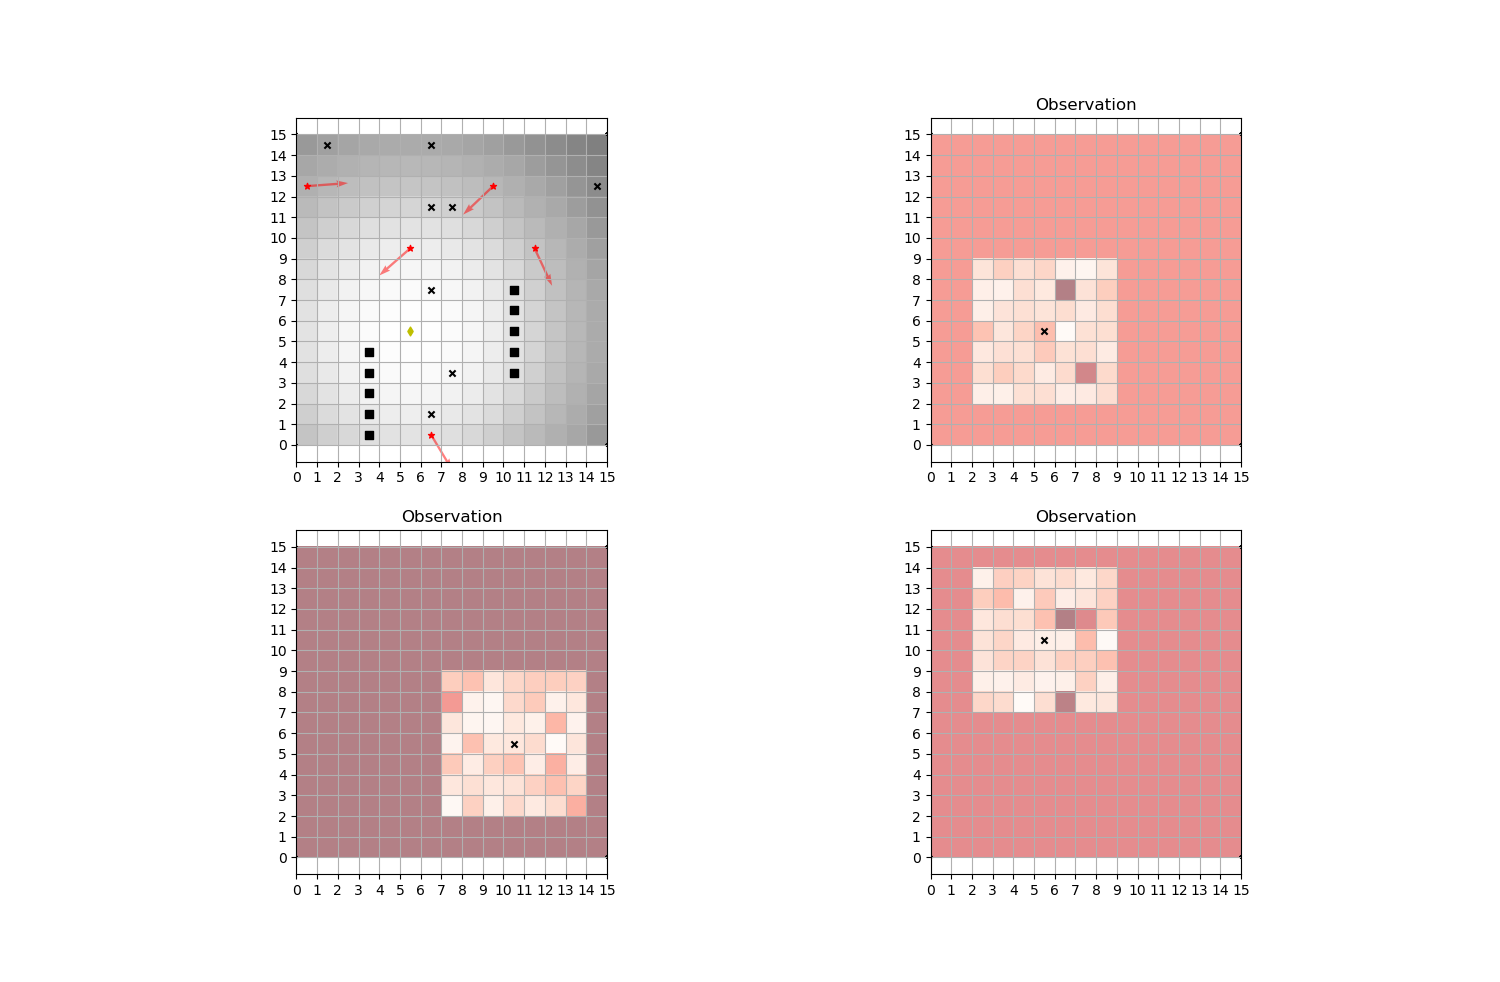
\includegraphics[width=0.7\linewidth, height=0.3\textheight]{../figures/exploring_field}
		\caption[Exploring the field]{This is an image of the field(top right). 'X' represent the object placment, and black squares the obstacels. The brightness corresponds to the light quantity in each cell. The red stars and arrows indicate aliased points, and the direction where aliasing is strongest. On the other plots a few observations are taken from different places, the color intensity corresponds to the probability of there being an object. Red = object, White = no object}
		\label{fig:exploringfield}
	\end{figure}

	\subsection{Qualitative experiments}
	\begin{figure}
		\centering
		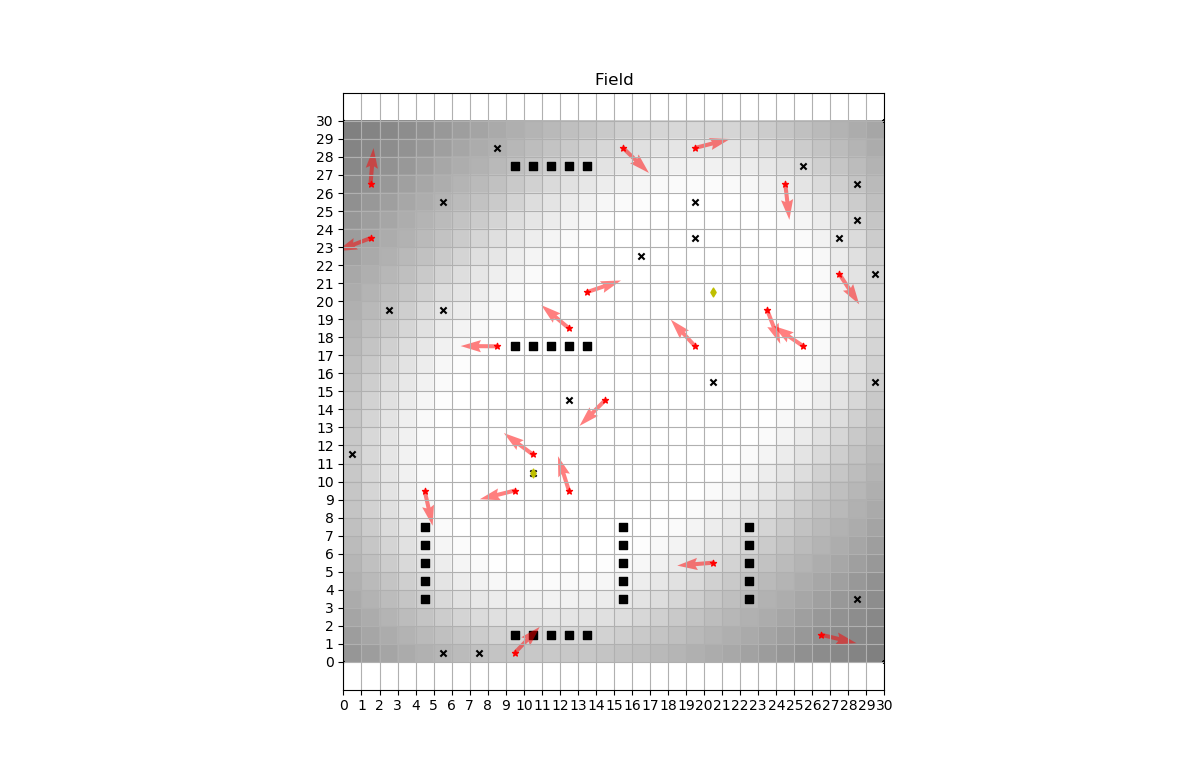
\includegraphics[width=0.7\linewidth, height=0.3\textheight]{../figures/ind_vs_corr_field_only}
		\caption[qualitative experiment field]{This is the field that the experiment run on}
		\label{fig:indvscorrfieldonly}
	\end{figure}
	\begin{figure}
		\centering
		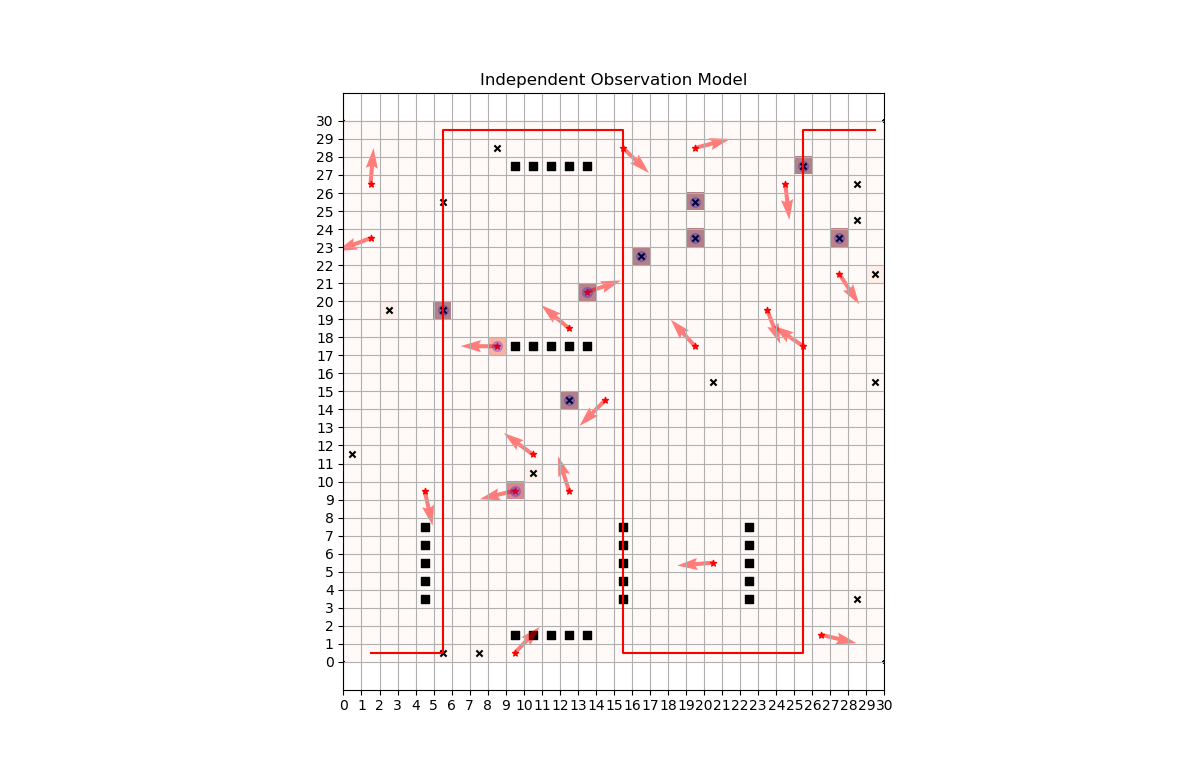
\includegraphics[width=0.7\linewidth, height=0.3\textheight]{../figures/ind_vs_corr_independent_agent}
		\caption[independent model results]{trajectory in red, red level indicates how certain the model is that there is an object at that point}
		\label{fig:indvscorrindependentagent}
	\end{figure}
	\begin{figure}
		\centering
		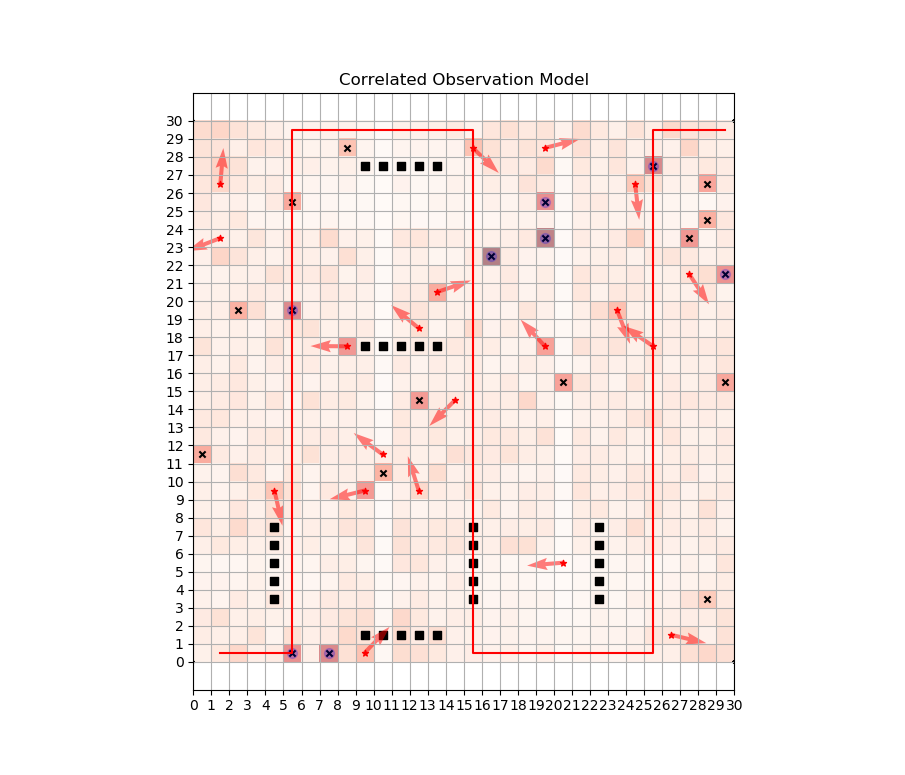
\includegraphics[width=0.7\linewidth, height=0.3\textheight]{../figures/ind_vs_corr_correlated_agent}
		\caption[Correlated model results]{same as independent}
		\label{fig:indvscorrcorrelatedagent}
	\end{figure}
	We can clearly see that the predictions in the independent model are much sharper, both on accurate ones and accurate ones, and that the correlated model is more conservative about it's estimation, and we can clearly see that even when it makes mistakes, it has some uncertainty to the results. 
	
	
	\subsection{Quantitative experiments}
	We run 5 experiments, using 5 different setting for the field, with raising complexity.  and for each field, we run 50 times, and average their results.
	overall we got pretty similar results with the correlated and uncorrelated model, probably because the correlated model parameters were roughly selected, but still we can see that the correlated models preforms slightly better then the independent model. The models are evaluated in terms of accuracy and MSDE.(see graphs)
	
	\begin{figure}
		\centering
		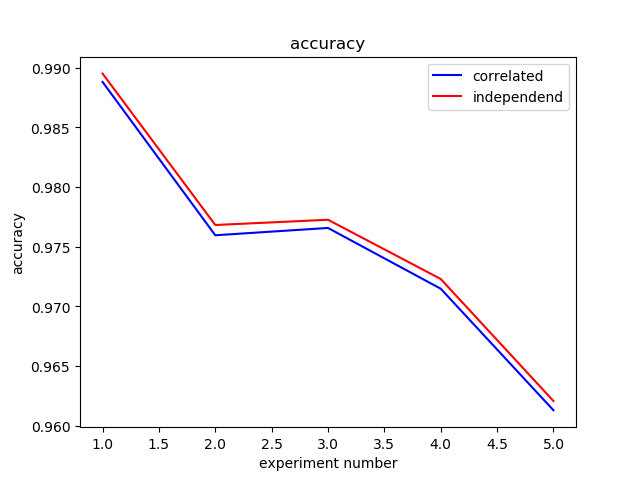
\includegraphics[width=0.7\linewidth, height=0.3\textheight]{../figures/accuracy_results}
		\caption[Accuracy results]{we can see that the correlated model slightly outpreforms the independent model}
		\label{fig:accuracyresults}
	\end{figure}
	\begin{figure}[h]
		\centering
		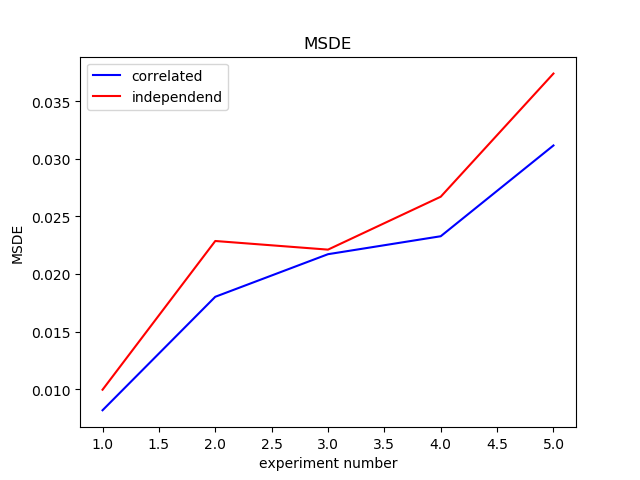
\includegraphics[width=0.7\linewidth, height=0.3\textheight]{../figures/MSDE_results}
		\caption[MSDE results]{we can see a more significant differance with the MSDE values.}
		\label{fig:msderesults}
	\end{figure}
	
	
	\section{Discussion and Conclusions}
	
	\subsection{Summery}
	In this report we examined 2 articles written on the subjects `active exploration` and `observation correlation modeling`,
	in the context of robust object detection. From the papers results we can clearly see useful to drop the assumption that observations are uncorrelated.
	Both in (a) planning and (b) observation modeling. Both papers give us methods that can be used for this, but probably too simplistic at their current form, and can be improved in future work.
	
	
	\subsection{Criticism}
	\textbf{Model Training} - both of the papers train their model on the exact(or very similar) environment of the testing experiment, but in most cases we cannot be guaranteed to have such training data available, and we will need to train our models in another surrounding, and try to generalize. The papers did not test to see how much does the learned model generalizes.  
	
	\subsection{Notes and Future Research}
	
	*\textbf{First of all} We want to incorporate what that we have learned in the course and the papers, and draw some conclusions.
	In the papers, the SLAM problem is assumed to be perfectly solved. That is usually not the case, we still have some uncertainty about the robot and objects locations. That increases the level of uncertainty in the classification with this method, because we use the robot's location in modeling the correlation, so when our location is uncertain, this will add to the total uncertainty.
	
	Another problem is that when our location and the object's relative location is uncertain, we will eventually get data association problems, i.e. thinking that 2 different objects are the same one, - this might lead to the wrong classification of at least one object(if they are not of the same class), with high uncertainty, even if the actual classifier preformed perfectly.
	or we can mistaken that one object is 2 different ones, this will lead to at least one false positive result.
	
	on the contrary, if we do not assume that SLAM is solved We can benefit from that.
	By incorporating all the observations, including the observed object's and their classes, we gain another layer of information to use in our optimization, this will give us more ways to check if our matches are correct, and to better estimate loop closers(accepting or rejecting), by using the extra information from class that might match or not. 
	
	the active exploration part can also be used to reduce uncertainty in the SLAM part of the problem.
	
	One of the possible data association problems that might arise is when the same object, because of slight drifts in pose estimation appears in 2 adjacent grid cells, this is very likely, and this destroys our assumption that different cells are uncorrelated.  \\
	
	Both papers assume that \textbf{different object hypothesis / grid cells are uncorrelated}, and only assume correlations between different observations of the same object / grid cell. even that it is usually not the case, in search and rescue it is reasonable to assume that victims will be next to each other, that a computer, a keyboard and a chair will probably come together, or as explained above, the same object might appear twice as 2 different objects due to bad data association, and we need to think how might we merge this 2 different hypothesis in the future if we gather more information that gets us better localization. It might be valuable not to neglect this correlation. \\
	
	\textbf{decisions are independent of path planning} - paper [2] assume that the decision actions(deciding is there an object in some place or not) is independent on the path planning, and could be done in the end. But what if 'is there an object' question's answer affects our objective / path planning? examples for that are: if the objects are things that we want to avoid like land-mines, or things that have meaning about the way we should move like traffic signs, or determine the objective, like finding a helipad to land on? It is valuable to tackle this question.	
  
\end{document}
